\documentclass[../main.tex]{subfiles}

\begin{document}

    \begin{figure}[H]
        \begin{center}
        \centerline{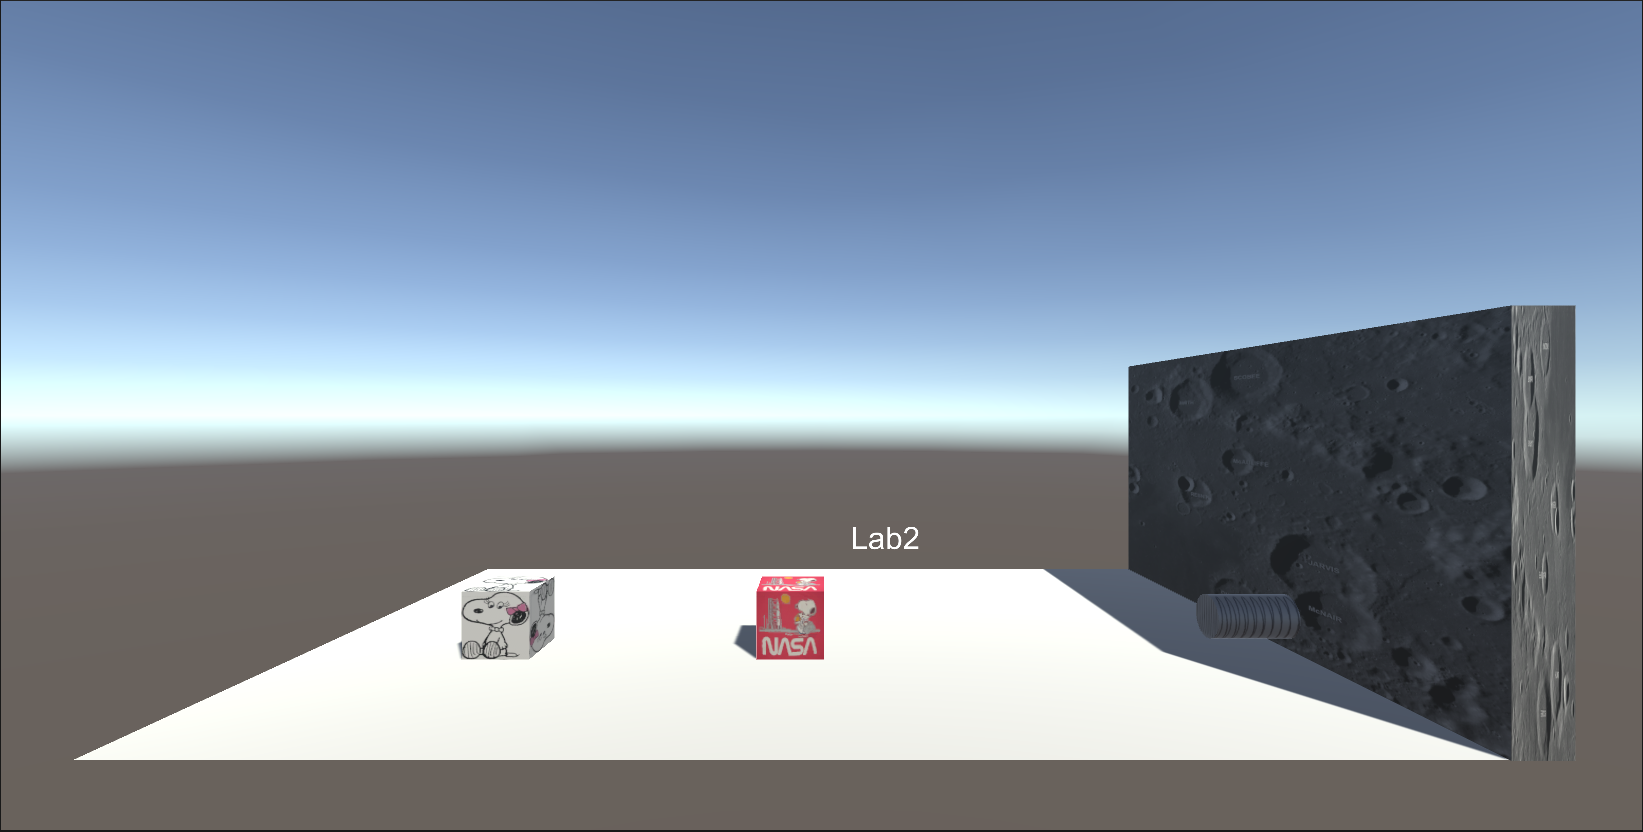
\includegraphics[width=155mm]{./images/2Lab_ExperimentOverview}}
            \caption{Experiment Übersicht}
            \label{fig:2Lab_ExperimentOverview}
        \end{center}
    \end{figure}
Im Code wird der Würfel, welcher am Anfang beschleunigt wird, Romeo benannt und der andere Würfel entsprechend
Julia. Die Würfel werden in den nächsten Abschnitten ebenfalls so bezeichnet, damit man denn Zusammenhang mit den
Screenshots des Codes leichter versteht. Zur Kontrolle der Werte und Grafik Erstellung wurde zwei verschiedene
CSV Datei erstellt (timeseries genannt), eine für den elastischen Stoss relevanten Werte und eine für den inelastischen Stoss.
\newline
Für die Beschleunigung von Romeo wird gemäss Berechnung, eine konstante Kraft von 4 (Newton) im FixedUpdate hinzugefügt.
Die Beschleunigunszeit von einer Sekunde wird von den Autoren bestimmt.
Der Würfel braucht also eine Sekunde um die maximale Geschwindigkeit zu erreichen.
Die konstante Kraft wirkt solange bis die Geschwindigkeit von 2m/s erreicht.
Dabei wird Romeo wird dann auch die kinetische Energie berechnet und in beiden Timeseries notiert.
\newline
Beim Teil mit dem elastischen Stoss wurde ein Feder GameObject hinzugefügt. Die Federkonstante wird am Start berechnet
bevor sich Romeo bewegt. Dies wird wie in der Berechnung erwähnt das Energieerhaltungsgesetz angewendet und für die
Federstauchung wurde 1.3 (Meter) gewählt, sodass der berechnete Federkonstante Wert 4.733 (N/m) beträgt. Beim Start
wird ebenfalls die Position der Feder in der Ruhelage, dort welche Romeo die Feder zuerst berühren würde, in der
Variable springMaxDeviation gespeichert.
\newline
Diese wird in FixedUpdate gebraucht um zu überprüfen, ob Romeo bereits auf die Feder eintrifft.
Sobald dies der Fall ist, verändert sich die Texture von Romeo und dann wird jeweils die Federkraft darin
berechnet und an Romeo hinzugefügt. Dafür wird der Längenunterschied der Feder mit der Differenz aus der
Position von Romeo und springMaxDeviation berechnet und danach mit der negativen Federkonstante multipliziert.
Dadurch bewegt sich Romeo  zurückt. Als Überprüfung der Energieerhaltung wird schlussendlich auch die potentiele
Energie der Feder berechnet und in der elastischen Timeseries zusammen mit der Federkraft aufgeschrieben.
\newline
Für den inelastischen Stoss mit Julia wird im OnCollisionEnter jeweils geprüft, ob es sich bei der Kollision um
Julia handelt. Nur wenn dies der Fall ist, wird dann ein FixedJoint an den Berührungspunkte zwischen Romeo und
Julia hinzugefügt um die damit sie zusammenkleben. Zum Schluss muss noch .enableCollision auf false gesetzt werden,
damit sich die beiden Würfeln nicht mehr kollidieren.
\newline
Im FixedUpdate wird dann für die inelastische Timeseries die Impulse berechnet und die gemeinsame Endgeschwindigkeit
und kinetische Energie. Mit dieser Geschwindigkeit kann dann auch die Kraft welche auf Julia wirkt errechnet werden.


    @kimmie: pls descibe
    - script in c#
    - klass erbt monobehavior
    --> bietet riged body, on bxo collieder, alle methoden die gebraucht werden
    - einezlne objekte
    - inelastisch fixejoint (screenshot)
    - erklärung warum spring gameobject und nicht rigedbody
    - screenshots von unity mit guggus infos :D
    - wenn uf code willsch iga:


  code uf bestimmti ziele:
    \begin{lstinputlisting}[label={lst:graphInelastic}, firstline=7, lastline=12]
    {..//UnityProj/Assets/CubeController.cs}
    \end{lstinputlisting}

    \begin{itemize}
        \item Julia:
        \begin{itemize}
            \item Material
            \item Cube
            \item Boxcolider enabled
            \item Contraints
            \item Frictionless
        \end{itemize}

        \item \item Romeo:
        \begin{itemize}
            \item Wall
            \item Lame
            \item Süffel
        \end{itemize}
    \end{itemize}

\end{document}